\chapter{The Impact of Genetic Drift on Selected Alleles}
\label{Selection_Stochasticity}
%\begin{quote}
%``Did he fire six shots or only five? [...] you've got to ask yourself
%one question'' `Do I feel lucky?' Well do ya, punk? '' -- Dirty Harry 
%\end{quote}

In the previous chapter we assumed that the selection acting on our
alleles was strong enough that we could ignore the action of genetic
drift in shaping allele frequency. However, genetic drift affects all
alleles, and so in this chapter we explore the interaction of
selection and drift. Strongly selected alleles can be
lost from the population via drift when they are rare in the population. While both weakly
beneficial and weakly deleterious alleles are subject to the random
whims of genetic drift throughout their entire time in the
population. Understanding the interaction of selection and genetic
drift is key to understanding the extent to which small populations
may be mutation-limited in their rate of adaptation, and how rates of
molecular and genome evolution may differ across taxa.
%In Chapter \ref{Chapter:Drift}

\section{Stochastic loss of strongly selected alleles}

% Fisher (1922, 1930) and Haldane (1927)
Even strongly beneficial alleles can be lost from the population when
they are sufficiently rare. This is because the number of offspring
left by individuals to the next generation is fundamentally
stochastic. A selection coefficient of s=$1\%$ is a strong
selection coefficient, which can drive an allele through the
population in a few hundred generations once the allele is
established. However, if individuals have on average a small number of
offspring per generation the first individual to carry our allele who
has on average $1\%$ more children could easily have zero offspring, leading to the loss
of our allele before it ever get a chance to spread.\\

To take a first stab at this problem lets think of a very large
haploid population and consider starting from a single individual with the selected allele, and ask
about the probability of eventual loss of our selected allele starting
from this single copy ($p_L$). To derive this we'll make use of a
simple argument \citep[derived from branching processes][]{fisher1923xxi,haldane1927mathematical}. Our selected
allele will be eventually lost from the population if every individual
with the allele fails to leave descendants.
\begin{figure}
\begin{center}
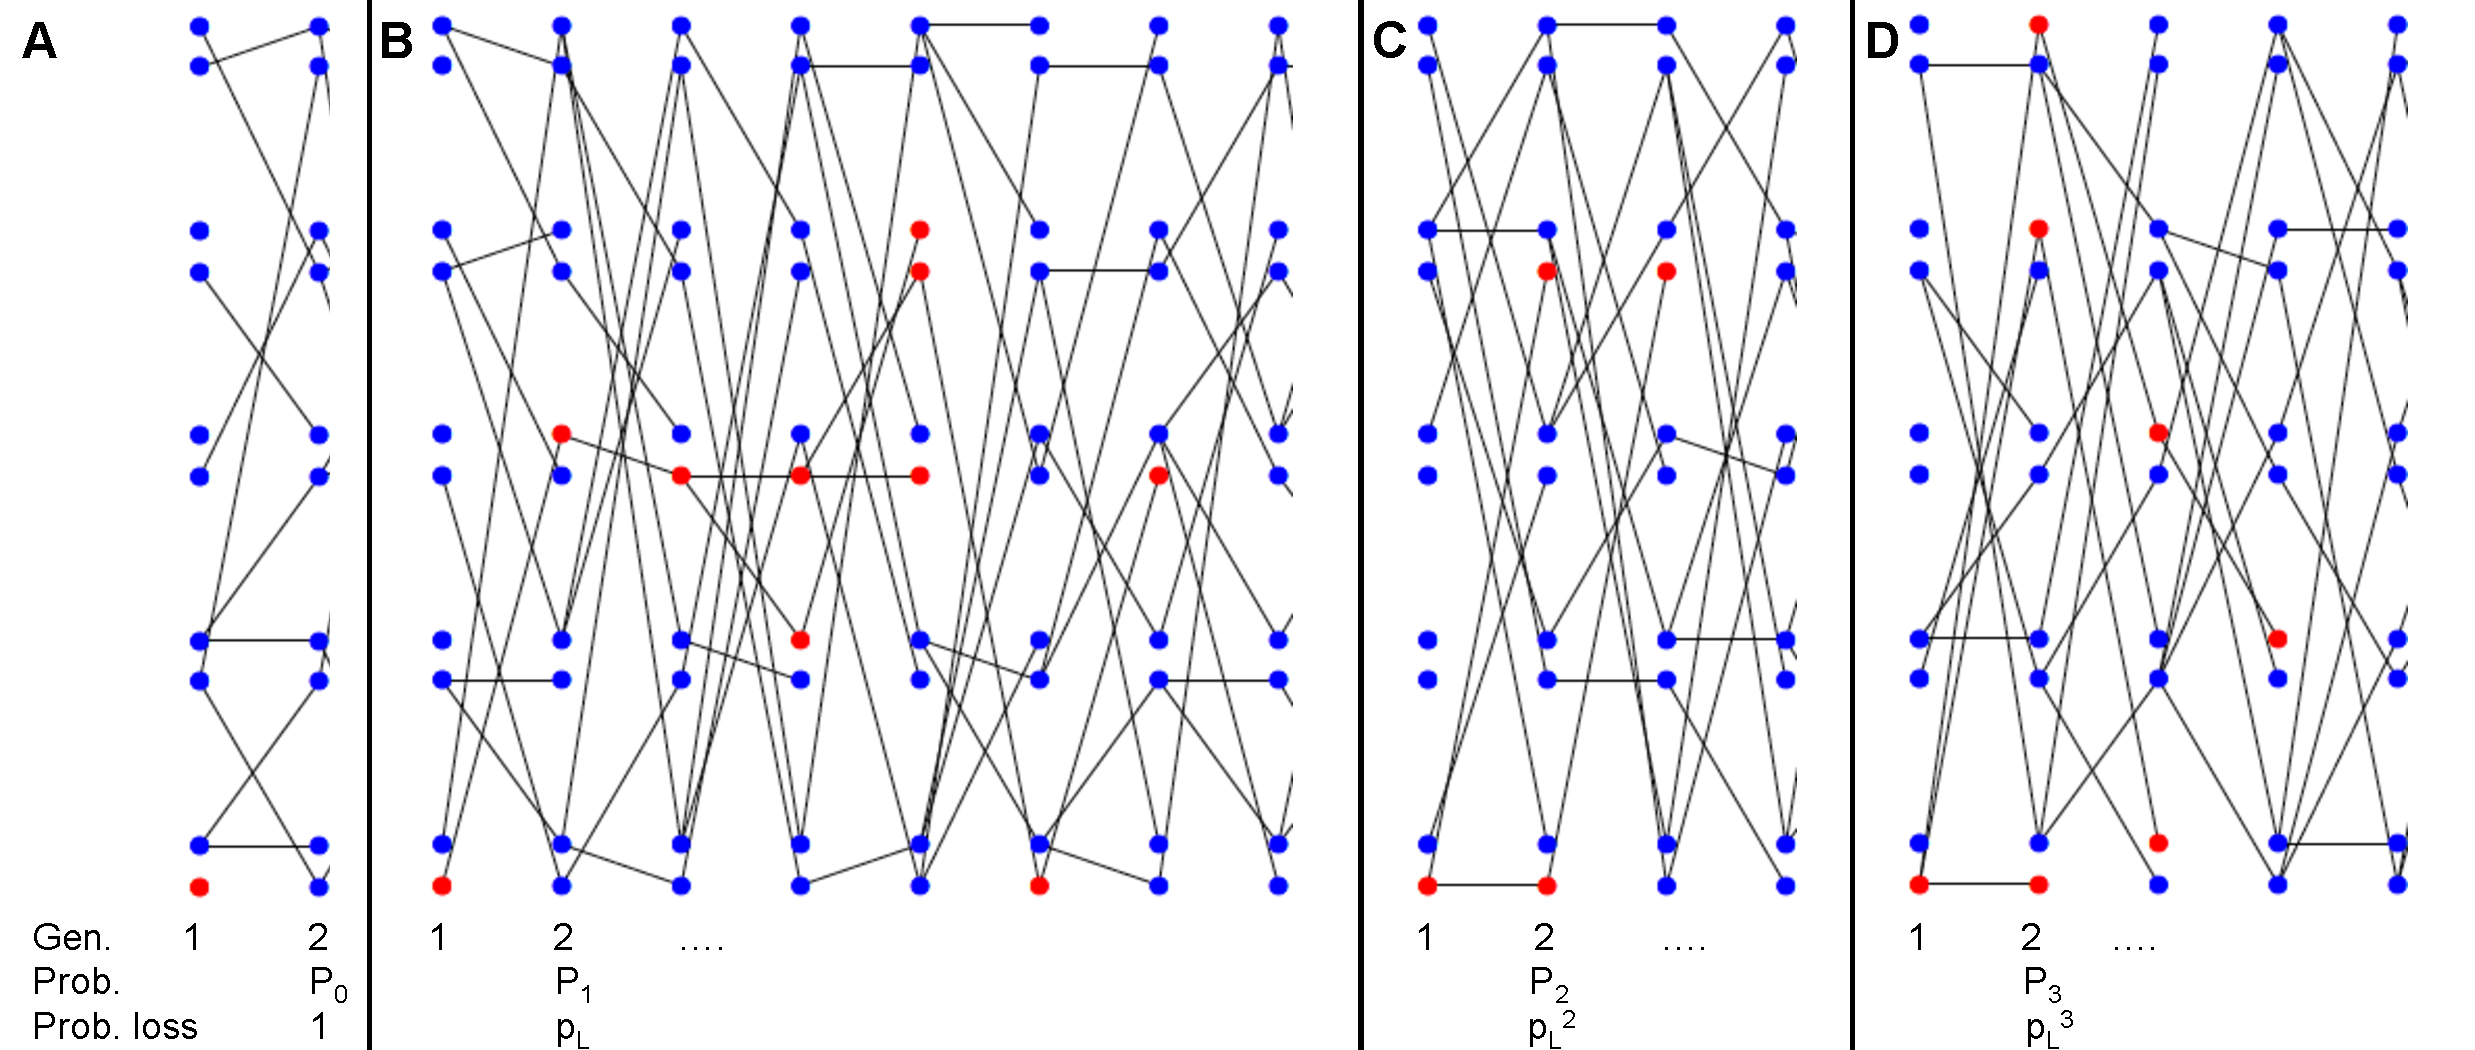
\includegraphics[width=\textwidth]{figures/Proof_of_pL_2s.pdf}
\end{center}
\caption{} \label{fig:Proof_of_pL_2s}
\end{figure}
Well we can think about different cases 
\begin{enumerate}
\item In our first generation
with probability $P_0$ our individual leaves no copies of itself to
the next generation, in which case our allele is lost (Figure \ref{fig:Proof_of_pL_2s}A).
\item Alternatively
it could leave one copy of itself to the next generation (with
probability $P_1$), in which
case with probability $p_L$ this copy eventually goes extinct (Figure \ref{fig:Proof_of_pL_2s}B).
\item It could leave two copies of itself to the next generation (with
probability $P_2$), in which
case with probability $p_L^2$ both of these copies eventually goes
extinct (Figure \ref{fig:Proof_of_pL_2s}C).
\item More generally it could leave could leave $k$ copies ($k>0$) of itself to the next generation (with
probability $P_k$), in which case with probability $p_L^k$  all of
these copies eventually go extinct (e.g. Figure \ref{fig:Proof_of_pL_2s}D).
\end{enumerate}
summing over these probabilities we see that
\begin{equation}
  p_L = \sum_{k=0}^{\infty} P_k p_L^{k}
\end{equation}
We'll now need to specific $P_k$, the probability that an individual
carrying our selected allele has $k$ kinds. In order for this population to stay constant in size
we'll assume that individuals without the selected mutation have on average one
offspring per generation, while individuals with our selected allele
have on average $1+s$ offspring per generation. We'll assume that the
distribution of offspring number of an individual is Poisson
distributed with mean $1+s$, i.e. the probability that an individual
with the selected allele has $i$ children is
\begin{equation}
P_i= \frac{(1+s)^i e^{-(1+s)}}{i!}
\end{equation}
Substituting this into the above we see
  \begin{align}
p_L &=  \sum_{k=0}^{\infty} \frac{(1+s)^ke^{-(1+s)}}{k!} p_L^{k} \nonumber
\\
&= e^{-(1+s)} \left( \sum_{k=0}^{\infty} \frac{\left(p_L(1+s) \right)^k}{k!}  \right)
\end{align}
well the term in the brackets is itself an exponential expansion, so
we can rewrite this as
\begin{equation}
p_L = e^{(1+s)(p_L-1)} \label{prob_loss}
\end{equation}
solving this would give us our probability of loss for any selection
coefficient. Lets
rewrite this in terms of the the probability of escaping loss $p_F = 1-p_L$.  We can
rewrite eqn \eqref{prob_loss} as
\begin{equation}
1-p_F = e^{-p_F(1+s)}
\end{equation}
to gain an approximation to this lets consider a small selection
coefficient $s \ll 1$ such that $p_F \ll 1$ and then expanded out the
exponential on the right hand side (ignoring terms of higher
order than $s^2$ and $p_F^2$) then
\begin{equation}
1-p_F \approx 1-p_F(1+s)+p_F^2(1+s)^2/2
\end{equation}
solving this we find that
\begin{equation}
p_F = 2s.
\end{equation}
Thus even an allele with a $1\%$ selection coefficient has a $98\%$
probability of being lost when it is first introduced into the
population by mutation. \\


%%consider reparameterizing 1+(1-hs)s
We can also adapt this result to a diploid setting.
Assuming that heterozygotes for the $1$ allele have $1+hs$ children, the
probability of allele $1$ is not lost, starting from a single copy in
the population, is
\begin{equation}
p_F = 2 h s \label{eqn:diploid_escape}
\end{equation}
for $h>0$. Note this is a slightly different parameterization from
our diploid model above, here $h$ is the dominance of out selected
allele with $h=1$ .\\


\begin{question}
Melanic squirrels suffer a higher rate of predation (due to hawks) than normally pigmented squirrels. Melanism is due to a dominant, autosomal mutation. The frequency of melanic squirrels at birth is $4 \times 10^{-5}$.\\

{\bf A)} If the mutation rate to new melanic alleles is $10^{-6}$,
assuming the melanic allele is at mutation-selection equilibrium, what
is the reduction in fitness of the heterozygote? \\ 
Suddenly levels of pollution increase dramatically in our population,
and predation by hawks now offers an equal (and opposite) advantage to
the dark individuals as it once offered to the normally pigmented
individuals. \\
{\bf B)} What is the probability that a single copy of this allele
(present just once in the population) is lost?\\ 
{\bf C)}  If the population size of our squirrels is a million
individuals, and is at mutation selection-balance, what is the probability that the population adapts from
anyone of these standing pool of melanic alleles?  
\end{question}

\section{The interaction between genetic drift and weak selection.}
For strongly selected alleles, once the allele has escaped initial
loss at low frequencies, their path will be determined deterministically by their
selection coefficients. However, if selection is weak compared to
genetic drift the stochasticity of reproduction can play a role in the trajectory an
allele takes even when it is common in the population. If selection is
sufficiently weak compared to genetic drift, then genetic drift will dominate the dynamics of alleles
and they will behave like they're effectively neutral. Thus the extent
to which selection can shape patterns of molecular evolution will
depend on the relative strengths of selection and genetic drift.


Asellid isopods have repeatedly invaded subterranean ground water from
surface water habitats many times. These ground water habitats are
more resource poor and so may
\citet{lefebure2017less} found \gc{that}

 \begin{figure}
 \begin{center}
 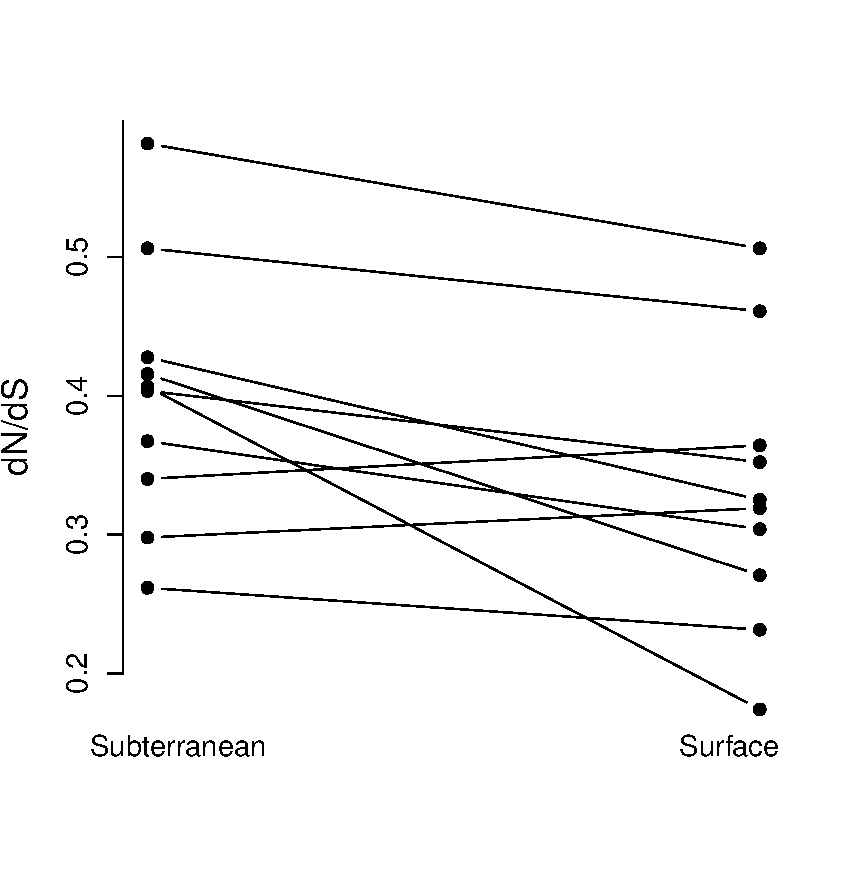
\includegraphics[width=\textwidth]{Journal_figs/drift_selection/asellid_isopods_Nes/asellid_isopods_Nes.pdf}
 \end{center}
 \caption{} \label{fig: asellid_isopods_Nes}
 \end{figure}

% \begin{figure}
% \begin{center}
% 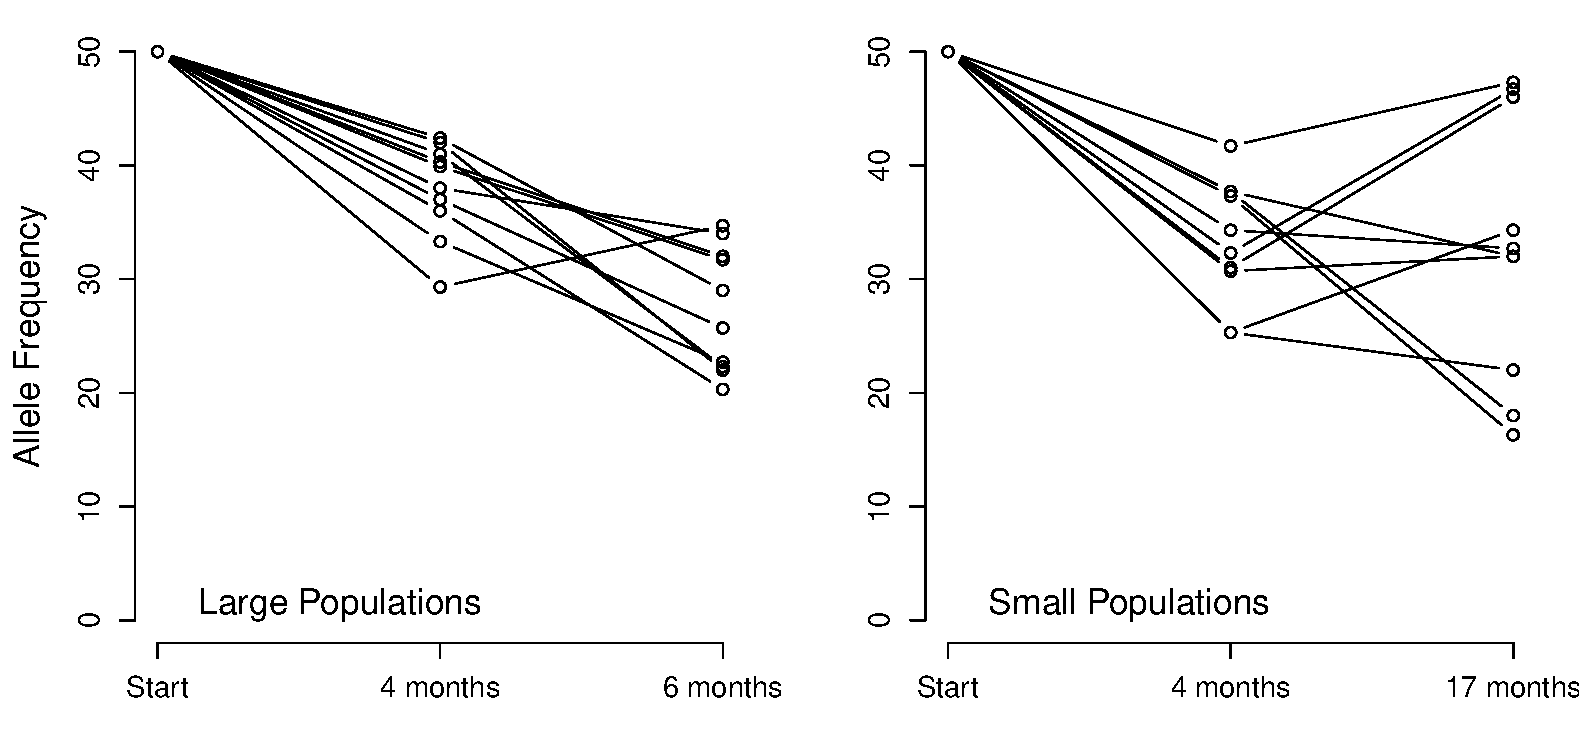
\includegraphics[width=\textwidth]{Journal_figs/drift_selection/DobPav/Drift_sel_Dobzhansky_Pavlovsky.pdf}
% \end{center}
% \caption{Data from \citet{dobzhansky1957experimental} } \label{fig:Dobzhansky_Pavlovsky}
% \end{figure}
% A classic case study of the interplay of genetic drift with selection is the
%  {\it Drosophila pseudoobscura} experiments of
% \citet{dobzhansky1957experimental}. \citeauthor{dobzhansky1957experimental} 
% setup multiple large populations each with 4000 indviduals and
% multiple small populations of 20
% individuals. They initiated each of these populations with the `Pikes
% Peak' (PP) inversion allele at $50\%$
% frequency.
% The PP allele was known to experience heterozygote advantage, with the
% PP homozygotes being less fit than the alternate homozygotes. In all of the
% large population cages moved relatively uniformly towards the
% equilbrium frequency. However, due to geneti drift in  

%To see this lets think of our simple Wright-Fisher model (see R
%exercise).

Each generation we allow a deterministic change in our
allele frequency, and then binomially sample two alleles for each of
our offspring to construct our next generation.

%%%%%Include this discussion of sampling back in our HWE section??
%%%%%Next time

So the expected change in our allele frequency within a generation is given just by our
deterministic formula. To make things easy on our self lets assume an
additive model, i.e. $h=1/2$, and that $s \ll 1$ so that $\wbar
\approx 1$. This gives us
\begin{equation}
\E(\Delta p ) = \frac{s}{2} p(1-p) \label{eqn:WF_mean}
\end{equation}
our variance in our allele frequency change is given by
\begin{equation}
Var(p^{\prime} - p) = Var(p^{\prime}) = \frac{p^{\prime}(1-p^{\prime})}{2N}
\end{equation}
this variance in our allele frequency follows from the fact that we
are binomially sampling $2N$ new alleles in the next
generation from a frequency $p^{\prime}$. Denoting our count of allele $1$ by $i$ our
\begin{equation}
Var(p^{\prime} - p) = Var(\frac{i}{2N} - p) =  Var(\frac{i}{2N} ) =\frac{Var(i)}{(2N)^2}
\end{equation}
and from binomial sampling $Var(i) = 2N p^{\prime}(1-p^{\prime})$ and
so we arrive at our answer. Assuming that $s \ll 1$, $p^{\prime}
\approx p$, then in practice we can use
\begin{equation}
Var(\Delta p)  =Var(p^{\prime} - p) \approx \frac{p(1-p)}{2N}. \label{eqn:WF_var}
\end{equation}
To get our first look at the relative effects of selection vs drift we
can simply look at when our change in allele frequency caused
selection within a generate is reasonably faithfully passed across
the generations. In particular if our expected change in frequency is much
great than the variance around this change, genetic drift will play
little role in the fate of our selected allele (once the allele is not
too rare within the population). When does selected
dominant genetic drift? This will happen if $\E(\Delta p) \gg Var(\Delta p)$ when $Ns \gg 1$. Conversely any
hope of our selected allele following its deterministic path will be quickly undone if our change in allele frequencies due to selection is
much less than the variance induced by drift. So if $Ns \ll 1$ then
drift will dominate the fate of our allele. \\
\begin{figure}
\begin{center}
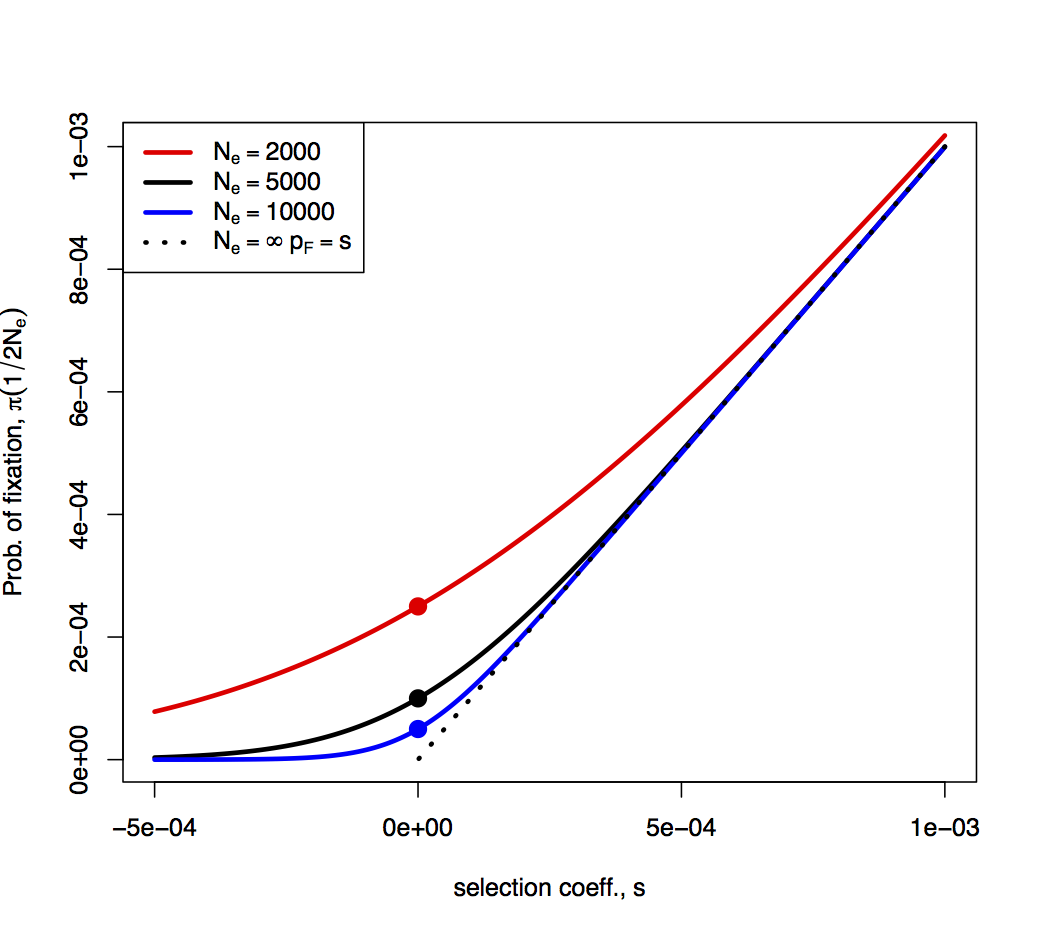
\includegraphics[width=0.6\textwidth]{figures/prob_fix_diffusion.png}
\end{center}
\caption{The probability of the fixation of a new mutation with
  selection coefficient $s$ ($h=1/2$) in a diploid population of effective
  size $N_e$. The dashed line gives the infinite population
  solution. The dots give the solution for $s \rightarrow 0$, i.e. $1/(2N_e)$} \label{fig:prob_fix_diffusion}
\end{figure}

To make further progress on understanding the fate of alleles with
selection coefficients of the order $1/N$ requires more careful
modeling. However, we can obtain the probability that under our diploid model, with an additive selection coefficient $s$, the
probability of allele $1$ fixing within the population starting
from a frequency $p$ is given by
\begin{equation}
\pi(p) = \frac{1-e^{-2Ns p }}{1-e^{-2Ns}} \label{eqn:prob_fixed}
\end{equation}
the proof of this is sketched out below (see Section \ref{Section:fixation_weakly_sel}). A new allele will arrive in the population at frequency $p=1/(2N)$,
then its probability of reaching fixation is
\begin{equation}
\pi \left(\frac{1}{2N} \right) = \frac{1-e^{-s }}{1-e^{-2Ns}} \label{eqn:new_mut_prob_fixed}
\end{equation}
if $s \ll1$ but $Ns \gg 1$ then $\pi(\frac{1}{2N}) \approx s$, which
nicely gives
us back our result that we obtained above
(eqn. \eqref{eqn:diploid_escape}). Our probability of fixation
(eqn. \eqref{eqn:new_mut_prob_fixed}) is plotted as a function of $s$
and $N$ in Figure \ref{fig:prob_fix_diffusion}. To recover our neutral
result we can take the
limit $s \rightarrow 0$ to obtain our neutral fixation
probability $1/(2N)$. \\

In the case where $Ns$ close to $1$ then
\begin{equation}
\pi \left( \frac{1}{2N} \right) \approx \frac{s}{1-e^{-2Ns}} \label{eqn:escape_from_intro}
\end{equation}
this is greater than our result $p_F=s$ from the branching process
argument (using our additive model of $h=1/2$), increasingly so for smaller $N$. 
Why is this?  The reason why is that $p_F$ is really the probability
of “never being lost” in an infinitely large population. So to persist
indefinitely the allele has to escape loss permanently, by never being
absorbed by the zero state. When the population size is finite, to fix
we only need to reach a size 2N individuals. Weakly beneficial
mutations (Ns~1) are slightly more likely to fix than the s
probability, as they only have to reach 2N to never be lost.


%Well in small populations selected alleles spend a
%somewhat shorter time segregating (especially at low frequencies), and so are
%slightly less susceptible to genetic drift. \\

\subsection{The fixation of slightly deleterious alleles.}
From Figure \ref{fig:prob_fix_diffusion} we can see that weakly
deleterious alleles can also fix, especially in small populations.  To understand how
likely it is that deleterious alleles accidently reach fixation by
genetic drift, lets assume a diploid model with additive selection (with
a selection coefficient of $-s$ against our allele $2$).  
If $N s \gg 1$ then our deleterious allele (allele $2$) can not possibly reach
fixation. However, if $Ns$ is not large then
\begin{equation}
\pi \left( \frac{1}{2N} \right) \approx \frac{s}{e^{2Ns}-1} \label{eqn:fix_deleterious}
\end{equation}
for our deleterious allele. So deleterious alleles can fix within
populations (albeit at a low rate) if $Ns$ is not too large. As above
this is because while deleterious mutations will never escape loss in
infinite population, but they can become fixed in finite population by
reach 2N copies. This is captured by the denominator of the fixation
probability under the diffusion model, which that this increases the
fixation prob. of alleles with absolute values of selection coefficients where |Ns|~1.

%The absorption of alleles at 2N

%copies can also be modeled in finite individual models (i.e. not the
%diffusion limit), but we will not go into that here. 

The ability of a population to avoid fixing weakly deleterious
mutations depends on the effective size of the population. 

\begin{figure}
\begin{center}
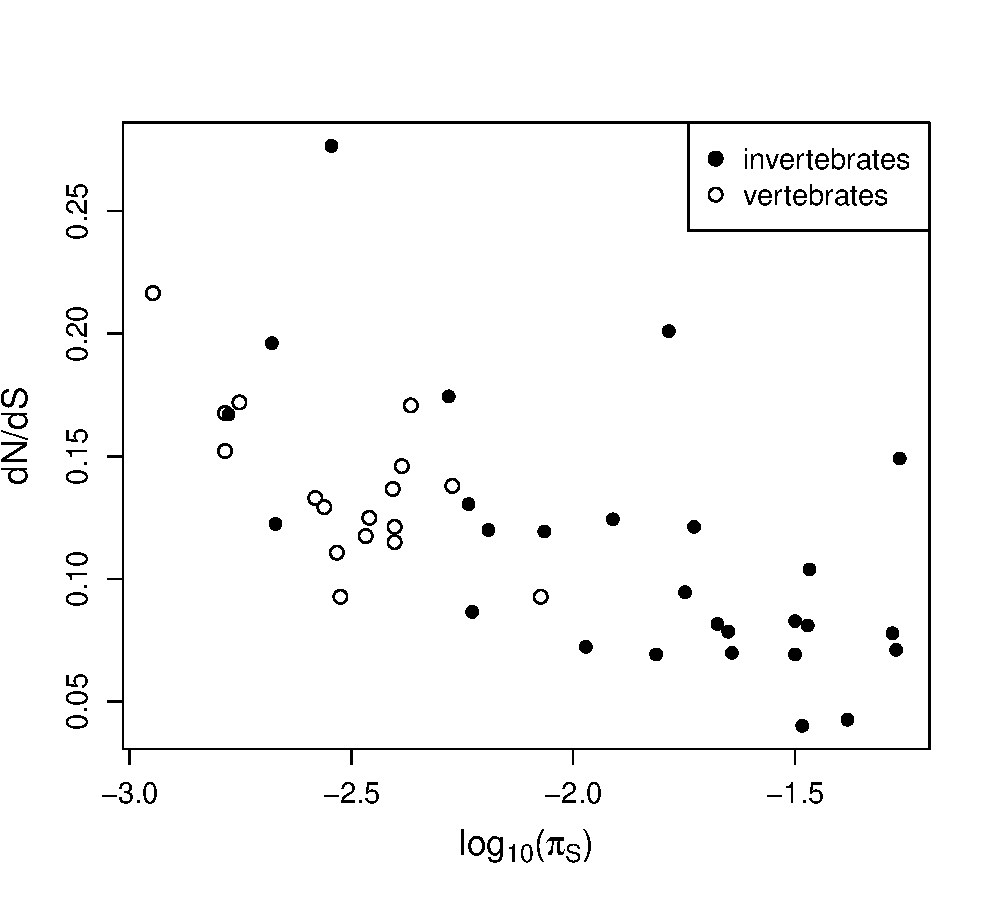
\includegraphics[width=\textwidth]{Journal_figs/drift_selection/Galtier_dNdS/Galtier_dNdS.pdf}
\end{center}
\caption{Data from \citet{galtier2016adaptive} } \label{Galtier_dNdS}
\end{figure}


\begin{marginfigure}
  \begin{center}
    
\includegraphics[width=0.6\textwidth]{figures/haldanes_sieve.png}
\end{center}
\caption{} \label{fig:haldanes_sieve}
\end{marginfigure}

\begin{question}
`Haldane's sieve' is the name for the idea that the mutations that contribute to adaptation are likely to be dominant or at least co-dominant. \\
{\bf A)} Briefly explain this argument with a verbal model relating to the
results we’ve developed in the last two chapters. \\
{\bf B)} Haldane’s sieve is thought to be less important for adaptation from previously deleterious standing variation, than adaptation from new mutation. Can you explain the intuition behind of this idea?\\
{\bf C)} Haldane’s sieve is likely to be less important in inbred,
e.g. selfing, populations. Why is this? \\

\end{question}




\subsection{A Sketch Proof of the probability of fixation of
weakly selected alleles} \label{Section:fixation_weakly_sel}
%Kolmogorov backward eqn. 1931
%Kimura, M. 1962 On the Probability of Fixation of Mutant Genes in a
%Population. for abitrary dominance in diffusion.

We'll let $P(\Delta p)$ be the probability that our allele frequency
shifts by $\Delta p$ in the next generation. Using this we can write our probability $\pi(p)$ in terms of the probability of
achieving fixation averaged over the frequency in the next generation
\begin{equation}
\pi(p)  = \int \pi(p+\Delta p) P(\Delta p) d(\Delta p) \label{eqn:prob_fix_diff_step1}
\end{equation}
This is very similar to the technique that we used deriving our
probability of escaping loss in a very large population above. \\

So we need an expression for $\pi(p+\Delta p)$. To obtain this we'll
do a Taylor series expansion of $\pi(p)$ assuming that $\Delta p $ is small
\begin{equation}
\pi(p+\Delta p) \approx \pi(p) + \Delta p \frac{d\pi(p)}{dp} + (\Delta p)^2
\frac{d^2\pi(p)}{dp^2} (p)
\end{equation}
ignoring higher order terms.\\

Taking the expectation over $\Delta p $ on both sides, as in
eqn. \ref{eqn:prob_fix_diff_step1}, we obtain
\begin{equation}
\pi(p) = \pi(p) + \E(\Delta p) \frac{d\pi (p)}{dp} + \E((\Delta p)^2)
\frac{d^2\pi(p)}{dp^2}
\end{equation}

Well $\E(\Delta p) = \frac{s}{2}p(1-p)$ and $Var(\Delta p)= \E((\Delta
p)^2)-\E^2(\Delta p)$, so if $s \ll 1$ then $\E^2(\Delta p) \approx
0$, and $\E(\Delta p)^2 = \frac{p(1-p)}{2N}$. This leaves us with
\begin{equation}
0= \frac{s}{2}p(1-p)\frac{d\pi (p) }{dp} + \frac{p(1-p)}{2N}
\frac{d^2\pi (p) }{dp^2}
\end{equation}
and we can specify the boundary conditions to be $\pi(1)=1$ and $\pi(0)=0$. 
Solving this differential equation is somewhat involved process but in
doing so we find that
\begin{equation}
\pi(p) = \frac{1-e^{-2Ns p }}{1-e^{-2Ns}}
\end{equation}
This proof can be extended
to alleles with arbitrary dominance, however, this does not lead to a
analytically tractable expression so we do not pursue this here. 

